% Provenance (never printed): see sources/outline_sources.md (Year 2: climate archives and proxies;
% foraminiferal and ice isotopes; Mg/Ca; pollen; speleothems; tree rings; dating the archives).
% Calibrations after Miller et al. (2020), Groeneveld et al. (2019) and Morley et al. (2024); ice
% cores after White (Geochemistry, ch. 9), Werner et al. (2018) and the EPICA Dome C file of Jouzel
% et al. (2007); age model after Svensson et al. (2008); deep-water context after Wharton et al.
% (2026); figures from figdata/bachelor-2/proxies.py (data/derived lr04, edc-temperature,
% co2-icecore); values of the exercises and problem computed in the Book 4 scratch calculator
% calc/ch24.py.
\chapter{Arquivos e indicadores climáticos}\label{ch:b2:climate-proxies}

Num artigo de 1955, um jovem geoquímico apresentou os isótopos de oxigênio das minúsculas carapaças de
foraminíferos retiradas de testemunhos do fundo oceânico, e encontrou neles quinze ciclos glacial--interglacial nos
últimos \num{600000} anos. Leu-os sobretudo como temperatura: atribuía apenas cerca de um quinto das
oscilações ao gelo armazenado em terra. Dezoito anos depois, Shackleton e Opdyke concluíram o
contrário: o efeito principal era o armazenamento de água isotopicamente leve nos mantos de
gelo. As mesmas carapaças, os mesmos números, duas leituras. Uma carapaça de calcita registra a
temperatura da água em que cresceu e a composição dessa água, e a composição da
água do mar depende de quanto gelo há em terra. Este capítulo trata desses registros, dos
arquivos que os guardam, dos indicadores lidos neles, de como são calibrados contra termômetros
e de como são datados, e da arte de separar dois sinais trazidos por uma só carapaça.
% ledger: white13c9:paleo-history

\begin{recall}
\textbf{Dos volumes escolares}: arquivo e \omterm{def:b2:climate-proxies:proxy}{indicador climático}, testemunho de gelo, período glacial e
interglacial, o Último Máximo Glacial (cerca de \num{23000} a \num{19000} anos atrás), a análise
polínica. \textbf{Do volume do primeiro ano}: a datação radiométrica, a idade radiocarbono e sua
curva de calibração; a vasa calcária, feita de cocólitos e de carapaças de foraminíferos.
\textbf{Do \cref{ch:b2:isotope-geochemistry}}: os padrões isotópicos de referência \omterm{def:b2:isotope-geochemistry:standards}{VSMOW} e \omterm{def:b2:isotope-geochemistry:standards}{VPDB}
(\cref{def:b2:isotope-geochemistry:standards}) e a \omterm{prop:b2:isotope-geochemistry:mwl}{reta da água meteórica}, $\delta\mathrm{D}
\approx 8\,\delta^{18}\mathrm{O} + 10$ (\cref{prop:b2:isotope-geochemistry:mwl}). \textbf{Dos
livros de química}: o valor $\delta$ e o fator de fracionamento. \textbf{Dos livros de
matemática}: a reta de mínimos quadrados.
\end{recall}
% ledger: ipcc:lgm-cooling, kc98:mwl, kc98:standards

\section{Arquivos e indicadores}\label{sec:b2:climate-proxies:archives}

Os instrumentos só medem o clima há pouco tempo. Tudo o que é anterior se lê em materiais
que cresceram ou se depositaram camada por camada enquanto o clima agia sobre eles: a neve que se transforma em gelo nos
mantos de gelo polares, as carapaças que chovem sobre o fundo oceânico, os anéis das árvores, os corais, os depósitos das
cavernas, a lama dos lagos. Os volumes escolares chamaram-nos arquivos, e as grandezas medidas
neles, indicadores; agora precisamos de palavras mais precisas.

\begin{definition}[Arquivo climático; indicador climático]\label{def:b2:climate-proxies:proxy}
Um \emph{arquivo climático}\index{arquivo climático} é um material natural que se acumula
progressivamente, camada sobre camada ou anel sobre anel, e conserva características físicas, químicas ou biológicas
do ambiente em que cada parte se formou. Um \emph{indicador
climático}\index{indicador climático} é uma grandeza medida num arquivo que depende de uma variável
climática, como uma temperatura, uma quantidade de chuva ou um volume de gelo, através de uma relação que pode
ser calibrada, e que faz assim as vezes de uma medição dessa variável que nunca foi feita.
\end{definition}
% ledger: ncei:proxy, ncei:paleocean

Três propriedades decidem o que um arquivo pode dizer: sua resolução (o intervalo de tempo coberto por uma
amostra), seu alcance (até onde recua no tempo) e a maneira como é datado. Um arquivo com camadas anuais pode ser
lido ano a ano e datado por contagem; os outros precisam de idades radiométricas ou da comparação com um
registro datado. A tabela abaixo compara os arquivos deste capítulo.

\begin{center}
\small
\begin{tabular}{>{\raggedright\arraybackslash}p{0.17\linewidth}>{\raggedright\arraybackslash}p{0.27\linewidth}>{\raggedright\arraybackslash}p{0.21\linewidth}>{\raggedright\arraybackslash}p{0.24\linewidth}}
\hline
arquivo & indicadores deste capítulo & camadas anuais & datação \\
\hline
sedimento de mar profundo & $\delta^{18}$O e Mg/Ca dos foraminíferos & não & radiocarbono, comparação com
registros datados \\
gelo polar & $\delta$D e $\delta^{18}$O do gelo, ar das bolhas & na parte superior dos testemunhos
espessos & contagem de camadas, camadas vulcânicas datadas \\
anéis de árvores & largura do anel, densidade da madeira, isótopos & sim & contagem e \omterm{def:b2:climate-proxies:dendro}{datação cruzada} dos anéis \\
\omterm{def:b2:climate-proxies:archives}{espeleotemas} & $\delta^{18}$O & em alguns & datação radiométrica \\
sedimentos lacustres & \omterm{def:b2:climate-proxies:archives}{varvas}, pólen & onde há \omterm{def:b2:climate-proxies:archives}{varvas} & contagem de \omterm{def:b2:climate-proxies:archives}{varvas} \\
\hline
\end{tabular}
\end{center}
% ledger: ncei:proxy, ncei:paleocean, ncei:tree-ring, ncei:speleothem, mccarthy23:varves, svensson08:gicc05, noaa:gisp2-layers, bebchuk26:crossdating

Um indicador nunca é uma medida pura de uma só variável. A largura de um anel de árvore depende do calor do
verão e da chuva; o $\delta^{18}$O de uma carapaça, da temperatura da água e de
sua composição isotópica. O trabalho do paleoclimatólogo é encontrar um indicador cuja dependência
da variável procurada seja forte e conhecida, medir as outras influências de modo independente, e
datar a amostra.

\section{Isótopos de oxigênio nas carapaças carbonáticas}\label{sec:b2:climate-proxies:oxygen}

Os foraminíferos são protistas unicelulares, muitos dos quais constroem uma carapaça de calcita; as espécies
planctônicas flutuam nas águas superficiais, as bentônicas vivem sobre o sedimento do fundo do mar ou dentro dele.
Suas carapaças acumulam-se nas vasas calcárias do volume do primeiro ano, e o
$\delta^{18}$O da calcita pode ser medido em algumas carapaças retiradas de cada centímetro de um
testemunho.
% ledger: ucmp:forams, ncei:paleocean

\begin{history}[Duas leituras de um registro]
Urey calculou em 1947 como o fracionamento do oxigênio entre a calcita e a água depende da
temperatura, e propôs que os carbonatos podiam registrar a temperatura em que se formaram. Cesare
Emiliani, então seu aluno, mediu o $\delta^{18}$O de foraminíferos de testemunhos de pistão dos
oceanos do mundo e publicou em 1955 um registro com 15 ciclos glacial--interglacial ao longo de
\num{600000} anos, atribuindo cerca de \qty{20}{\percent} da variação ao volume de gelo.
Em 1973 Shackleton e Opdyke concluíram que o armazenamento de água isotopicamente leve nos
mantos de gelo era o efeito principal. Os efeitos vitais, os desvios de uma espécie em relação ao equilíbrio,
e a troca de oxigênio com a água intersticial depois do soterramento em geral não são muito importantes para as
carapaças dos últimos milhões de anos; a composição isotópica da água é.
\end{history}
% ledger: white13c9:paleo-history

\subsection*{A temperatura}

A calcita que cresce em equilíbrio com a água é mais rica em \textsuperscript{18}O que a água,
e quanto mais fria a água, maior o enriquecimento, como mostrou o cálculo de Urey. Várias
calibrações empíricas relacionam
a temperatura à diferença entre o $\delta^{18}$O da calcita, na escala \omterm{def:b2:isotope-geochemistry:standards}{VPDB}, e
o da água, na escala \omterm{def:b2:isotope-geochemistry:standards}{VSMOW}. Para o mar profundo, usa-se uma forma simplificada para as carapaças
bentônicas.

\begin{proposition}[Uma calibração bentônica]\label{prop:b2:climate-proxies:benthic}
Para os foraminíferos bentônicos às temperaturas do mar profundo (abaixo de cerca de \qty{13}{\celsius}),
\[
  T = 16.1 - 4.76\,\bigl[\delta^{18}\mathrm{O}_{\mathrm{b}} - (\delta^{18}\mathrm{O}_{\mathrm{sw}} -
  0.27)\bigr],
\]
com $T$ em \unit{\celsius}, $\delta^{18}\mathrm{O}_{\mathrm{b}}$ o valor da carapaça (por mil,
\omterm{def:b2:isotope-geochemistry:standards}{VPDB}) e $\delta^{18}\mathrm{O}_{\mathrm{sw}}$ o da água do mar (por mil, \omterm{def:b2:isotope-geochemistry:standards}{VSMOW}); o termo
0.27 converte a água para a escala da calcita. Um resfriamento de \qty{1}{\celsius} com composição da
água constante eleva $\delta^{18}\mathrm{O}_{\mathrm{b}}$ em $1/4.76 = 0.21$ por mil.
\end{proposition}
\admitted
% ledger: miller20:paleotemp, groeneveld19:anand

A equação mais completa da qual ela é simplificada traz um pequeno termo quadrático,
$T = 16.1 - 4.64x + 0.09x^2$, sendo $x$ a diferença dos dois valores $\delta$; as carapaças planctônicas
têm suas próprias calibrações, da mesma forma, como $T = 14.9 - 4.8\,[\delta^{18}\mathrm{O} -
(\delta^{18}\mathrm{O}_{\mathrm{sw}} - 0.27)]$. Todas partilham uma dificuldade: a carapaça dá um só
número, $\delta^{18}\mathrm{O}_{\mathrm{b}}$, e a equação tem duas incógnitas, $T$ e
$\delta^{18}\mathrm{O}_{\mathrm{sw}}$. É preciso um segundo indicador, independente, para separá-las.
% ledger: miller20:paleotemp, groeneveld19:anand

\subsection*{O efeito do volume de gelo}

A água que evapora do mar leva menos \textsuperscript{18}O que o mar; à medida que o vapor
viaja para o polo e cai como chuva ou neve, empobrece-se ainda mais, e a neve que forma os mantos
de gelo está entre as águas mais leves do planeta: o gelo da Groenlândia tem um $\delta^{18}$O de $-30$ a $-35$
por mil, o gelo antártico chega a $-50$. Quando os mantos de gelo crescem, o isótopo leve fica preso em terra
e o oceano que resta torna-se mais pesado.
% ledger: nasaeo:o18, white:d18o

\begin{definition}[Efeito do volume de gelo]\label{def:b2:climate-proxies:ice-volume}
O \emph{efeito do volume de gelo}\index{efeito do volume de gelo} é a variação da composição isotópica do
oxigênio do oceano inteiro causada pelo crescimento ou pelo recuo dos mantos de gelo continentais, que
armazenam água empobrecida em \textsuperscript{18}O; ele desloca o $\delta^{18}$O de todo carbonato
formado no mar na mesma quantidade, qualquer que seja a temperatura.
\end{definition}
% ledger: nasaeo:o18, white13c9:ice-volume, miller20:paleotemp

\begin{omfigure}
\centering
\begin{tikzpicture}[font=\scriptsize, >=Stealth]
\foreach \col/\title in {0/{a\enspace hoje}, 7.0/{b\enspace um máximo glacial}} {
  \begin{scope}[shift={(\col,0)}]
  \node[anchor=south west] at (0,3.3) {\textbf{\title}};
  \fill[brown!30] (3.6,0) -- (6.4,0) -- (6.4,1.6) -- (3.6,1.2) -- cycle;
  \end{scope}
}
% today: full ocean, small ice sheet
\fill[ocBlue!25] (0,0) rectangle (3.6,1.2);
\node[align=center] at (1.75,0.55) {oceano\\$\delta^{18}\mathrm{O} = 0$};
\fill[white, draw=black!50] (5.2,1.43) .. controls (5.6,1.95) and (6.2,1.95) .. (6.4,1.6) -- cycle;
\node at (5.0,0.65) {gelo, $-40$};
\draw[black!50] (5.0,0.85) -- (5.7,1.55);
\draw[->, thick, ocBlue] (1.6,1.35) .. controls (2.4,2.9) and (4.6,2.9) .. (5.6,2.05);
\node at (3.4,3.0) {vapor, leve};
% glacial: lower sea, big ice sheet
\begin{scope}[shift={(7.0,0)}]
\fill[ocBlue!35] (0,0) rectangle (3.6,0.85);
\draw[densely dashed] (0,1.2) -- (3.6,1.2);
\node[anchor=south west, align=left] at (0.05,1.2) {nível do\\mar atual};
\draw[<->] (3.35,0.85) -- (3.35,1.2);
\node[anchor=east] at (3.3,1.02) {\qty{130}{m}};
\node[align=center] at (1.6,0.42) {oceano, $\delta^{18}\mathrm{O} = +1.46$};
\fill[white, draw=black!50] (3.6,1.2) .. controls (4.0,2.6) and (6.0,2.7) .. (6.4,1.6) -- cycle;
\node at (5.1,1.85) {gelo, $-40$};
\draw[->, thick, ocBlue] (2.15,0.9) .. controls (2.3,2.6) and (3.3,3.0) .. (4.3,2.6);
\end{scope}
\end{tikzpicture}
\par\smallskip{\small O \omterm{def:b2:climate-proxies:ice-volume}{efeito do volume de gelo} (esquemático, fora de escala): o vapor que alimenta os mantos
de gelo é empobrecido em \textsuperscript{18}O, de modo que armazenar \qty{130}{m} de nível do mar como gelo de
$\delta^{18}\mathrm{O} = -40$ por mil deixa o oceano \num{1.46} por mil mais pesado
(\cref{prop:b2:climate-proxies:mass-balance}). Valores em por mil, \omterm{def:b2:isotope-geochemistry:standards}{VSMOW}.}
\end{omfigure}
% ledger: nasaeo:o18, miller20:ice-cal, ipcc:lgm-sea

Qual é o tamanho do deslocamento? Um balanço de massa responde, se o volume do gelo e sua composição
isotópica média forem conhecidos.

\begin{proposition}[Efeito do volume de gelo por balanço de massa]\label{prop:b2:climate-proxies:mass-balance}
Suponha-se que o oceano atual tenha uma profundidade média $H$ e um $\delta^{18}$O de 0 (\omterm{def:b2:isotope-geochemistry:standards}{VSMOW}). Se uma camada de água
do mar de espessura $h$ for retirada e armazenada em terra como gelo de composição média
$\delta_{\mathrm{ice}}$, mantida fixa a área do oceano, o oceano restante tem
\[
  \Delta\delta^{18}\mathrm{O}_{\mathrm{sw}} = \frac{-h\,\delta_{\mathrm{ice}}}{H - h}.
\]
Para $h$ pequeno o deslocamento cresce quase linearmente, $-\delta_{\mathrm{ice}}/H$ por metro de nível do mar.
\end{proposition}

\begin{proof}
Para um isótopo minoritário, os valores $\delta$ combinam-se como concentrações: o $\delta$ de uma mistura é
a média dos valores $\delta$ de suas partes ponderada por suas quantidades de oxigênio, e todas as
partes aqui são água. Por unidade de área do oceano, a água do oceano atual, uma coluna $H$ com
$\delta = 0$, reparte-se entre o gelo, $h$ com $\delta_{\mathrm{ice}}$, e o oceano restante,
$H - h$ com $\Delta\delta^{18}\mathrm{O}_{\mathrm{sw}}$:
$H \times 0 = h\,\delta_{\mathrm{ice}} + (H - h)\,\Delta\delta^{18}\mathrm{O}_{\mathrm{sw}}$, o que
dá a fórmula. Para $h \ll H$, $H - h \approx H$.
\end{proof}
% ledger: white13c9:ice-mass, charette:ocean-volume

\begin{example}[O oceano do último glacial]\label{ex:b2:climate-proxies:lgm}
No Último Máximo Glacial o nível do mar estava 125 a \qty{134}{m} abaixo do atual; tome-se \qty{130}{m},
com $H = \qty{3682.2}{m}$, e gelo a $-40$ por mil, o valor inferido para o grande manto de gelo
norte-americano. Então
$\Delta\delta^{18}\mathrm{O}_{\mathrm{sw}} = 130 \times 40/(3682.2 - 130) = 5200/3552.2 = 1.46$
por mil, cerca de $40/3682.2 = 0.0109$ por mil por metro de nível do mar. As comparações com curvas do nível do mar
obtidas de terraços e recifes de coral datados dão \num{0.011} por mil por metro, em concordância; uma escala de
\num{0.13} por mil por \qty{10}{m}, usada em algumas reconstruções, corresponde a um gelo a cerca de
$-50$ por mil. Uma medição direta da variação, a partir do $\delta^{18}$O da água ainda retida
nos poros do sedimento glacial, dá $1.0 \pm 0.1$ por mil.
\end{example}
% ledger: ipcc:lgm-sea, charette:ocean-volume, miller20:ice-cal, white13c9:ice-volume, wharton26:deep

A figura abaixo mostra quanto a resposta depende da composição suposta para o gelo.
A diferença entre \num{1.0} e \num{1.5} por mil não é pequena: a \num{0.21} por mil por grau,
ela vale mais de dois graus de temperatura do oceano profundo. A relação também não é bem
linear: o oceano que resta diminui à medida que o gelo cresce, e o $\delta^{18}$O médio do próprio gelo
muda à medida que mantos de gelo de composições diferentes crescem e recuam. As reconstruções do nível do mar
a partir do $\delta^{18}$O usam por isso muitas vezes uma relação linear calibrada no valor da água intersticial,
reconhecendo ao mesmo tempo que a relação verdadeira deveria ser não linear.
% ledger: wharton26:deep, rohling21:linear, miller20:paleotemp

\begin{omfigure}
\centering
% figdata/bachelor-2/proxies.py part icevol
\begin{tikzpicture}
\begin{axis}[width=0.86\linewidth, height=6.0cm, xmin=0, xmax=150, ymin=0, ymax=2.2,
  xlabel={água do mar armazenada como gelo, $h$ (\unit{m} de nível do mar)},
  ylabel={$\Delta\delta^{18}\mathrm{O}_{\mathrm{sw}}$ (por mil)},
  tick label style={font=\scriptsize}, label style={font=\small}, xtick={0,25,...,150},
  legend style={font=\scriptsize, at={(0.5,1.02)}, anchor=south, draw=none, legend columns=4,
  /tikz/every even column/.append style={column sep=6pt}}, legend cell align=left]
\fill[black!10] (axis cs:125,0) rectangle (axis cs:134,2.2);
\addplot[ocBlue, thick] table[x=h_m, y=d30] {figdata/out/bachelor-2-proxies-icevol.dat};
\addlegendentry{gelo a $-30$}
\addplot[black, thick] table[x=h_m, y=d40] {figdata/out/bachelor-2-proxies-icevol.dat};
\addlegendentry{gelo a $-40$}
\addplot[ocRed, thick] table[x=h_m, y=d50] {figdata/out/bachelor-2-proxies-icevol.dat};
\addlegendentry{gelo a $-50$}
\addplot[only marks, mark=square*, mark size=1.8pt, omDef, error bars/.cd, y dir=both,
  y explicit] coordinates {(130,1.0) +- (0,0.1)};
\addlegendentry{água intersticial}
\addplot[black!60, densely dashed, domain=0:150, samples=2, forget plot] {1.69};
\node[font=\scriptsize, anchor=south west] at (axis cs:3,1.69) {variação total do LR04, 1.69};
\node[font=\scriptsize, anchor=north, align=center] at (axis cs:112,0.45) {último máximo\\glacial
$\rightarrow$};
\end{axis}
\end{tikzpicture}
\par\smallskip{\small O \omterm{def:b2:climate-proxies:ice-volume}{efeito do volume de gelo} pelo balanço de massa da
\cref{prop:b2:climate-proxies:mass-balance}, para três composições do gelo (por mil, \omterm{def:b2:isotope-geochemistry:standards}{VSMOW});
faixa cinza: a descida do nível do mar do Último Máximo Glacial, 125 a \qty{134}{m}; quadrado: a variação
medida nas águas intersticiais dos sedimentos, $1.0 \pm 0.1$ por mil, colocada em \qty{130}{m}; tracejado: a
variação da compilação bentônica entre hoje e o Último Máximo Glacial.}
\end{omfigure}
% ledger: ipcc:lgm-sea, wharton26:deep, data:b4-proxies, miller20:ice-cal

\subsection*{A compilação bentônica}

Os registros de $\delta^{18}$O bentônico de muitos testemunhos, alinhados e somados em média, formam uma compilação (stack) cujo ruído
é menor que o de qualquer testemunho isolado. A compilação LR04 combina 57 registros de locais espalhados pelo
oceano mundial e cobre 5.3 milhões de anos. Entre hoje, \num{3.23} por mil, e a média de
\num{19} a \qty{23}{ka}, \num{4.92} por mil, ela varia \num{1.69} por mil, mais do que qualquer
efeito de volume de gelo plausível. Como concluíram Shackleton e Opdyke, a maior parte da variação é o gelo;
mas restam alguns décimos de por mil para o resfriamento da água profunda. O problema deste capítulo mede esse resíduo.
% ledger: lr04:stack, data:b4-proxies, white13c9:paleo-history, wharton26:deep

\begin{omfigure}
\centering
% figdata/bachelor-2/proxies.py parts lr04, edc, co2
\begin{tikzpicture}
\begin{groupplot}[group style={group size=1 by 3, vertical sep=0.35cm, xlabels at=edge bottom,
  xticklabels at=edge bottom},
  width=0.96\linewidth, height=3.7cm, xmin=0, xmax=800, xtick={0,100,...,800},
  tick label style={font=\scriptsize}, label style={font=\small}]
\nextgroupplot[ylabel={$\delta^{18}\mathrm{O}_{\mathrm{b}}$}, y dir=reverse, ymin=2.45, ymax=5.2,
  ytick={3.5,4.5}]
\addplot[omDef, thin] table[x=age_ka, y=d18O] {figdata/out/bachelor-2-proxies-lr04.dat};
\node[font=\scriptsize, anchor=north east] at (rel axis cs:0.99,0.97) {a\enspace compilação LR04 (por
mil, VPDB; eixo invertido)};
\nextgroupplot[ylabel={$\Delta T$ (\unit{\celsius})}, ymin=-12, ymax=7, ytick={-10,-5,0,5}]
\addplot[ocBlue, thin] table[x=age_ka, y=dT] {figdata/out/bachelor-2-proxies-edc.dat};
\node[font=\scriptsize, anchor=north east] at (rel axis cs:0.99,0.97) {b\enspace anomalia de temperatura
de EPICA Dome C};
\nextgroupplot[ylabel={CO$_2$ (\unit{ppm})}, ymin=160, ymax=330, ytick={200,250,300},
  xlabel={idade (milhares de anos antes de 1950)}]
\addplot[ocRed, thin] table[x=age_ka, y=co2] {figdata/out/bachelor-2-proxies-co2.dat};
\node[font=\scriptsize, anchor=north east] at (rel axis cs:0.99,0.97) {c\enspace CO$_2$ do
ar dos testemunhos de gelo antárticos};
\end{groupplot}
\end{tikzpicture}
\par\smallskip{\small Os últimos \num{800000} anos em três arquivos: (a) a compilação bentônica de
$\delta^{18}$O LR04, traçada com o eixo invertido para que os tempos glaciais apontem para baixo; (b) a
anomalia de temperatura em EPICA Dome C, em relação à média do último milênio, deduzida
do $\delta$D do gelo; (c) o CO$_2$ do ar aprisionado no gelo antártico, até 1950. Dados: NOAA
NCEI Paleoclimatology (Lisiecki e Raymo 2005; Jouzel e colaboradores 2007; Bereiter e colaboradores 2015),
obtidos em 22 de outubro de 2026.}
\end{omfigure}
% ledger: data:lr04, data:edc-jouzel, data:co2-bereiter, jouzel07:edc-corr, data:b4-proxies

\section{Testemunhos de gelo}\label{sec:b2:climate-proxies:ice}

A neve que cai sobre um manto de gelo conserva a composição isotópica que tinha ao cair, e quanto
mais frio o lugar e a época, mais leve ela é. Na Antártida a temperatura média anual do ar e
o $\delta^{18}$O da neve seguem uma forte relação linear de um sítio para outro, com uma
inclinação de cerca de \num{0.8} por mil por grau, como prevê a destilação de Rayleigh do vapor em seu caminho
para o interior. O hidrogênio é usado tanto quanto o oxigênio: na \omterm{prop:b2:isotope-geochemistry:mwl}{reta da água meteórica}, $\delta$D varia cerca de oito vezes mais depressa que $\delta^{18}$O, e
o registro de $\delta$D do gelo antártico foi escolhido por sua maior sensibilidade à temperatura.
% ledger: werner18:slopes, white13c9:icecore, kc98:mwl

Uma inclinação medida no espaço não é necessariamente uma inclinação no tempo. Na Groenlândia, onde a própria
temperatura do gelo foi reconstruída por outros métodos, a variação de $\delta^{18}$O por grau
ao longo do tempo revela-se de 0.3 a \num{0.6} por mil, contra uma inclinação espacial atual de cerca de
\num{0.7}: as estações de queda de neve, as fontes da umidade e seus trajetos mudaram com o
clima. As primeiras temperaturas antárticas foram calculadas com uma relação espacial medida na
neve; as mais recentes usam modelos de circulação geral que simulam os isótopos da água.
% ledger: werner18:slopes, white13c9:icecore

O testemunho de EPICA Dome C, perfurado através de \qty{3260}{m} de gelo, chega a \num{800000} anos. Seu
$\delta$D foi medido em amostras de \qty{55}{cm} de comprimento, com uma exatidão de \num{0.5} por mil, e
convertido numa anomalia de temperatura em relação à média do último milênio, depois de
corrigido da composição variável da água do mar que alimentou a neve e da altitude variável
do manto de gelo. Entre os tempos glaciais e interglaciais a temperatura variou cerca de
\qty{15}{\celsius}. Entre os últimos dois mil anos e o Último Máximo Glacial (\num{19} a
\qty{23}{ka}), o $\delta$D médio cai de $-396.6$ para $-441.7$ por mil e a anomalia de
$-0.09$ para \qty{-9.39}{\celsius}.
% ledger: white13c9:icecore, jouzel07:edc-corr, jouzel07:edc, data:b4-proxies

O gelo também guarda ar. O firn, a neve compactada das primeiras dezenas de metros, está aberto para a
atmosfera até que seus poros se fechem na transição para o gelo, 50 a \qty{120}{m} abaixo; o ar
de uma bolha é portanto mais jovem que o gelo à sua volta. Medido nas bolhas, o CO$_2$ do
ar era em média de \qty{189.7}{ppm} entre \num{19} e \qty{23}{ka}, e de \qty{279.4}{ppm} nos
dois mil anos anteriores à indústria. Os painéis (b) e (c) da figura acima sobem e descem
juntos ao longo dos últimos \num{800000} anos.
% ledger: firn:close-off, data:b4-proxies-co2, data:co2-bereiter

Os testemunhos da Groenlândia chegam apenas a cerca de \num{120000} anos, mas a neve acumula-se ali mais depressa e
o registro é mais fino; ele mostra os aquecimentos abruptos do último período glacial conhecidos como
eventos de Dansgaard--Oeschger. Perto do topo de um testemunho espesso, as próprias estações podem ser vistas.
% ledger: white13c9:icecore

\begin{omfigure}
\centering
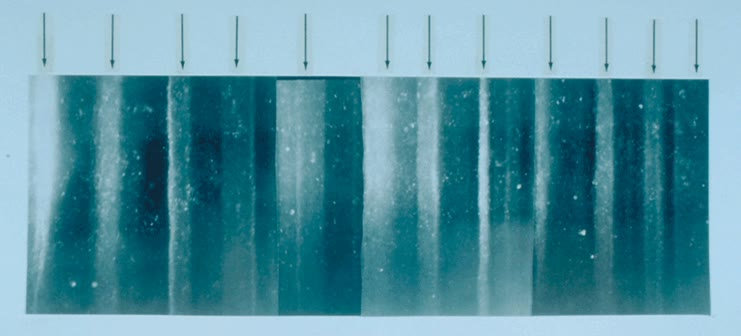
\includegraphics[width=0.72\linewidth]{images/book4/b2-24-gisp2-layers.jpg}
\par\smallskip{\small Uma seção do testemunho de gelo GISP2 do centro da Groenlândia a \qty{1855}{m}
de profundidade, iluminada por baixo, com camadas alternadas de verão e de inverno (as setas são as do
diapositivo original). Durante o seco verão boreal, a poeira do Ártico canadense e da costa da Groenlândia é
levada pelo vento para o manto de gelo.
(Anthony Gow, U.S.\ Army Corps of Engineers CRREL, coleção de diapositivos NOAA Paleoclimatology,
domínio público, via Wikimedia Commons.)}
\end{omfigure}
% ledger: photo:b2-24-gisp2, noaa:gisp2-layers

\begin{inthelab}[Cortar um testemunho de gelo]
\begin{minipage}[t]{0.54\linewidth}\vspace{0pt}
Num centro nacional de testemunhos de gelo, os testemunhos são guardados em tubos, um metro de testemunho por tubo, numa
câmara frigorífica de arquivo a \qty{-36}{\celsius}; os cientistas trabalham numa sala de exame a
\qty{-24}{\celsius}. Quando chega um novo testemunho, forma-se uma linha de processamento: cientistas e
técnicos medem, catalogam e cortam cada seção, tipicamente 30 a \qty{35}{m} por dia, de modo que um
testemunho de \qty{1000}{m} leva seis a oito semanas. Um pesquisador alisa o testemunho com uma
plaina e mede sua condutividade elétrica, uma chave para definir e datar as camadas; outro
serra os pedaços cujo ar aprisionado será analisado quanto ao dióxido de carbono e ao metano; as amostras são
então enviadas aos laboratórios que as medem. Em EPICA Dome C, cada amostra do perfil de $\delta$D
tinha \qty{55}{cm} de gelo.
\end{minipage}\hfill
\begin{minipage}[t]{0.42\linewidth}\vspace{0pt}
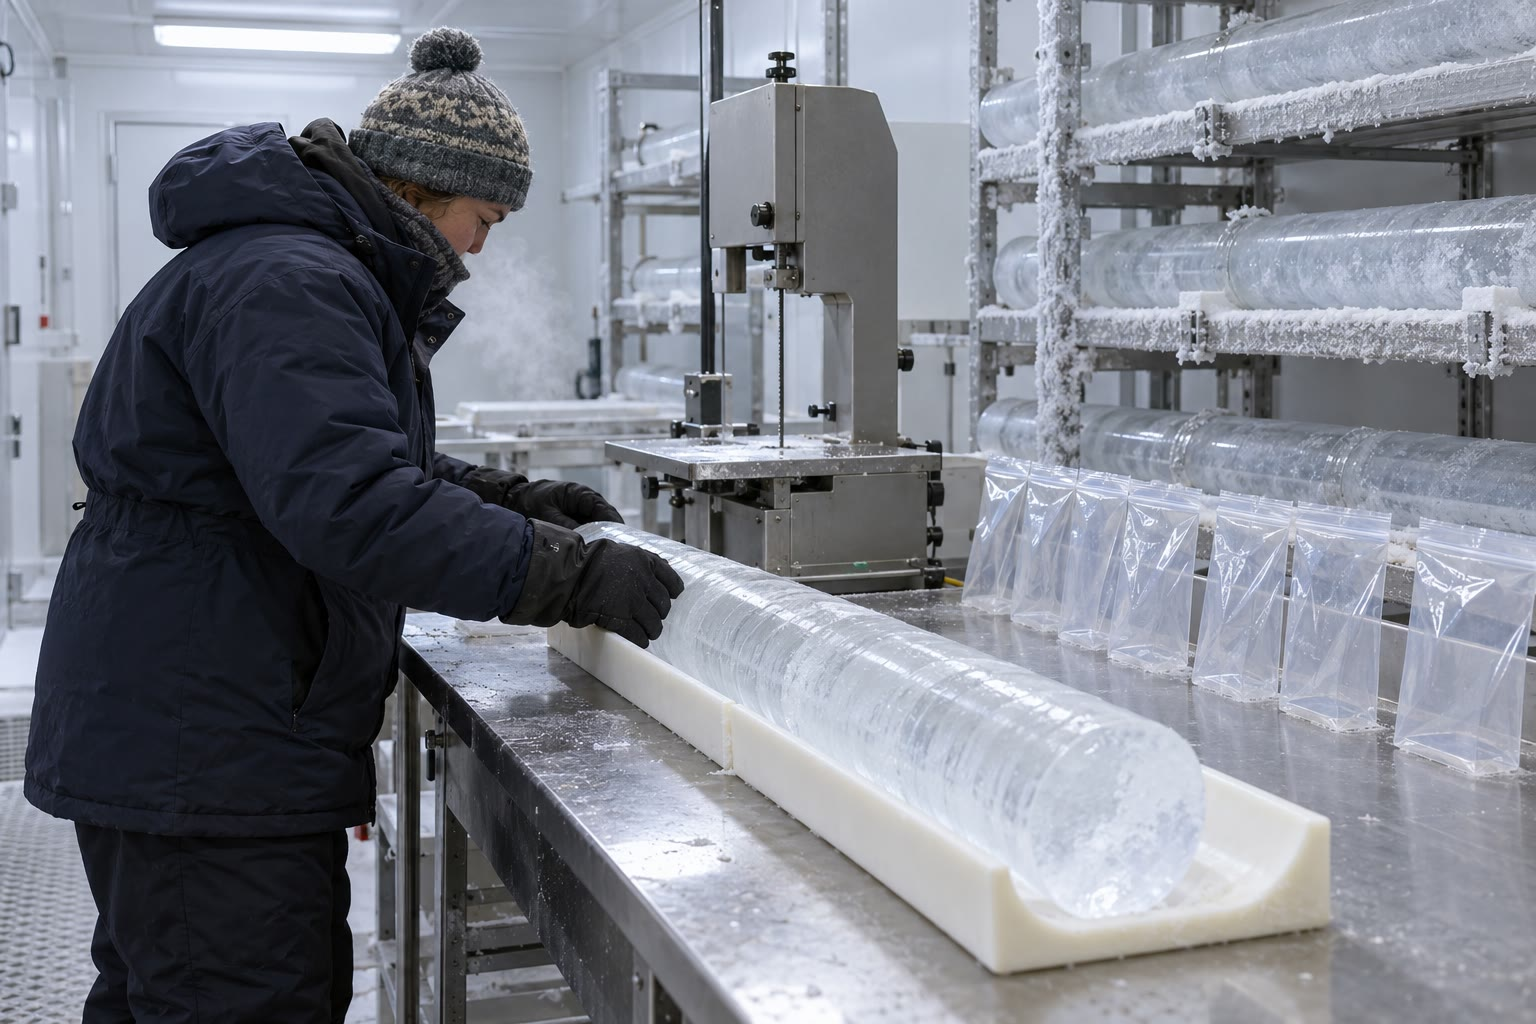
\includegraphics[width=\linewidth]{images/book4/ai/b2-24-cold-lab.jpg}

{\scriptsize Um pedaço de testemunho de gelo na bancada de um laboratório frio, ao lado de uma serra de fita e de sacos de
amostras (ilustração gerada por IA).}
\end{minipage}
\end{inthelab}
% ledger: nsficf:cpl, jouzel07:edc-corr

\section{Outros indicadores, outros arquivos}\label{sec:b2:climate-proxies:others}

\subsection*{O magnésio das carapaças}

A calcita dos foraminíferos incorpora um pouco de magnésio no lugar do cálcio, e mais quando
a água está mais quente. A razão não depende da composição isotópica da água, de modo que
dá a temperatura de que a equação do $\delta^{18}$O precisa.

\begin{definition}[Razão Mg/Ca (indicador)]\label{def:b2:climate-proxies:mgca}
A \emph{razão Mg/Ca (indicador)}\index{razão Mg/Ca (indicador)} é a razão entre o magnésio e o cálcio
na calcita das carapaças de foraminíferos, em \unit{mmol/mol}, usada como medida da temperatura da
água em que a carapaça cresceu através de uma calibração exponencial
\[
  \text{Mg/Ca} = B\,\mathrm{e}^{A T},
\]
com $A$ próximo de \qty{0.09}{\per\celsius} para as espécies planctônicas e $B$ próprio de cada espécie.
\end{definition}
% ledger: groeneveld19:anand, morley24:mgca, miller20:paleotemp

Com $A = 0.09$ a razão cresce $\mathrm{e}^{0.09} - 1 = \qty{9.4}{\percent}$ por grau,
qualquer que seja a temperatura. Para uma espécie planctônica de águas frias, a calibração prevista a partir
só da temperatura é $\text{Mg/Ca} = 0.4\,\mathrm{e}^{0.09T}$; um ajuste a 235 carapaças de redes de
plâncton e de topos de testemunhos do Atlântico Norte dá $0.372\,\mathrm{e}^{0.0936T}$, com $r^2 = 0.90$.
Às baixas temperaturas as razões medidas afastam-se da curva, e o desvio é atribuído à
concentração de íon carbonato na água do mar: um indicador raramente depende de uma só variável.
As espécies bentônicas são menos sensíveis, cerca de \qty{0.1}{mmol/mol} por grau para as espécies
pobres em magnésio que vivem no sedimento.
% ledger: morley24:mgca, wharton26:deep

\begin{omfigure}
\centering
% figdata/bachelor-2/proxies.py part calib
\begin{tikzpicture}
\begin{groupplot}[group style={group size=2 by 1, horizontal sep=1.7cm},
  tick label style={font=\scriptsize}, label style={font=\small}, height=5.2cm,
  width=0.48\linewidth]
\nextgroupplot[xmin=-2, xmax=14, ymin=0, ymax=3.8, xlabel={$T$ (\unit{\celsius})},
  ylabel={$\delta^{18}\mathrm{O}_{\mathrm{b}} - \delta^{18}\mathrm{O}_{\mathrm{sw}}$ (por mil)},
  xtick={0,4,...,12}, title={a\enspace $\delta^{18}$O bentônico}, title style={font=\scriptsize}]
\addplot[black, thick] table[x=T, y=dd_benthic] {figdata/out/bachelor-2-proxies-calib.dat};
\nextgroupplot[xmin=0, xmax=30, ymin=0, ymax=6.5, xlabel={$T$ (\unit{\celsius})},
  ylabel={razão Mg/Ca (\unit{mmol/mol})}, xtick={0,5,...,30}, title={b\enspace Mg/Ca planctônico},
  title style={font=\scriptsize},
  legend style={font=\scriptsize, at={(0.03,0.97)}, anchor=north west, draw=none},
  legend cell align=left]
\addplot[ocRed, thick] table[x=T, y=mgca_pred] {figdata/out/bachelor-2-proxies-calib.dat};
\addlegendentry{$0.4\,\mathrm{e}^{0.09T}$}
\addplot[ocBlue, thick, densely dashed] table[x=T, y=mgca_fit]
  {figdata/out/bachelor-2-proxies-calib.dat};
\addlegendentry{$0.372\,\mathrm{e}^{0.0936T}$}
\end{groupplot}
\end{tikzpicture}
\par\smallskip{\small Duas calibrações. (a) A calibração bentônica da
\cref{prop:b2:climate-proxies:benthic}: a calcita é mais pesada que a água (cada uma em sua
escala) \num{0.21} por mil a mais para cada grau de resfriamento. (b) A razão Mg/Ca de uma espécie
planctônica, prevista só a partir da temperatura e ajustada a 235 carapaças.}
\end{omfigure}
% ledger: miller20:paleotemp, morley24:mgca

Medidas nas mesmas carapaças, Mg/Ca e $\delta^{18}$O dão duas equações para duas incógnitas: Mg/Ca
dá $T$, e a \cref{prop:b2:climate-proxies:benthic} dá então
$\delta^{18}\mathrm{O}_{\mathrm{sw}}$, o sinal do volume de gelo. Aplicado a carapaças bentônicas do
Atlântico Noroeste profundo, o método encontra a água do Último Máximo Glacial apenas cerca de
\qty{2}{\celsius} mais fria que a atual ($-1.78 \pm \qty{0.56}{\celsius}$), enquanto as estimativas a partir das
águas intersticiais situam as duas massas de água profundas perto do congelamento no oceano glacial, $-1.1$ e
\qty{-1.9}{\celsius}, onde hoje estão a 2 a \qty{4}{\celsius} e 0 a \qty{1}{\celsius}.
% ledger: miller20:paleotemp, wharton26:deep

\subsection*{Os anéis das árvores}

\begin{definition}[Dendroclimatologia; datação cruzada]\label{def:b2:climate-proxies:dendro}
A \emph{dendroclimatologia}\index{dendroclimatologia} é a reconstrução do clima passado a partir dos
anéis de crescimento anuais das árvores: sua largura, a densidade de sua madeira e sua composição
isotópica. A \emph{datação cruzada}\index{datação cruzada} é a correspondência do padrão de anéis largos e
estreitos entre árvores, que atribui a cada anel seu ano civil absoluto e revela
anéis localmente ausentes numa árvore isolada.
\end{definition}
% ledger: bebchuk26:crossdating, bebchuk26:absent-rings, ncei:tree-ring, ncei:proxy

Um anel é mais largo quando as condições favorecem o crescimento. A \omterm{def:b2:climate-proxies:dendro}{datação cruzada} é confiável nos sítios de clima extremo, onde um só
fator climático limita o crescimento de todas as árvores, de modo que elas partilham o mesmo padrão; ela pode
falhar onde nenhum fator domina, e onde muitos anéis estão localmente ausentes.
Sobrepondo os padrões de árvores vivas, de madeiras antigas e de lenho soterrado, estende-se uma cronologia para trás
ano a ano; um estudo recente datou uma cronologia de 100 teixos subfósseis do leste da Inglaterra nos
456 anos de 2668 a 2213 a.C., usando o $\delta^{18}$O de mais de \num{1500} de seus anéis
contra uma cronologia de carvalhos datada de forma absoluta. O International Tree-Ring Data Bank reúne as larguras
de anéis, densidades, isótopos e cronologias de mais de \num{5000} sítios em seis continentes.
% ledger: ncei:proxy, bebchuk26:crossdating, bebchuk26:absent-rings, ncei:tree-ring

\subsection*{Cavernas e lagos}

\begin{definition}[Espeleotema; varva]\label{def:b2:climate-proxies:archives}
Um \emph{espeleotema}\index{espeleotema} é um depósito mineral formado a partir da água subterrânea dentro de uma
caverna: estalagmites, estalactites e outras formas. Uma \emph{varva}\index{varva} é
o depósito de um ano num sedimento de fundo de lago ou de mar, em geral um par de lâminas de composição
contrastante, uma depositada no verão e outra no resto do ano.
\end{definition}
% ledger: ncei:speleothem, mccarthy23:varves

Os \omterm{def:b2:climate-proxies:archives}{espeleotemas} crescem camada por camada a partir da água subterrânea que chega a uma caverna; a espessura de
suas camadas e seus registros isotópicos dão as condições climáticas passadas. Alguns têm bandas anuais,
e alguns contêm compostos que podem ser datados radiometricamente. A escala de tempo dos testemunhos da Groenlândia concorda com a dos
\omterm{def:b2:climate-proxies:archives}{espeleotemas} da caverna de Hulu com diferença de até 800 anos ao longo dos últimos \num{60000} anos: dois
arquivos, datados por métodos diferentes, verificam-se um ao outro.
% ledger: ncei:speleothem, svensson08:gicc05

\begin{omfigure}
\centering
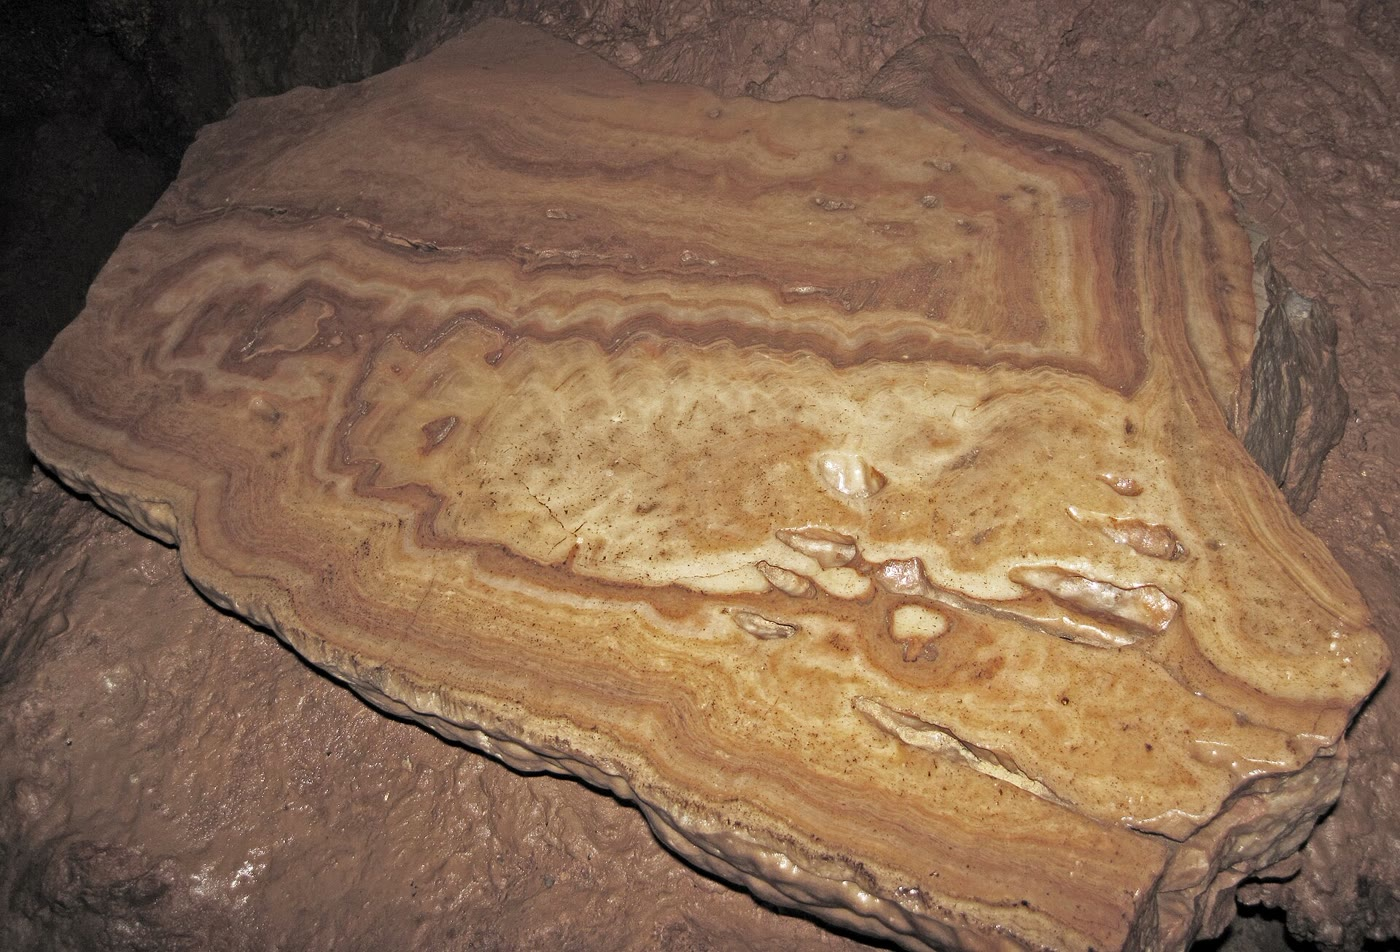
\includegraphics[width=0.62\linewidth]{images/book4/b2-24-speleothem.jpg}
\par\smallskip{\small Seção cortada e polida de um \omterm{def:b2:climate-proxies:archives}{espeleotema} de calcita de Diamond Caverns,
Kentucky, colorido por impurezas de óxido de ferro: cada banda foi um dia a superfície do depósito.
(Fotografia de James St.~John, CC BY 2.0, via Wikimedia Commons.)}
\end{omfigure}
% ledger: photo:b2-24-speleothem

Na bacia profunda do lago Crawford, em Ontário, a água do fundo, mais salgada e mais alcalina que
a água acima dela, não abriga animais grandes o bastante para revolver a lama, embora seja bem
oxigenada, e cada ano acrescenta um par: uma camada de matéria orgânica, coberta pela
calcita que precipita cada verão da água superficial alcalina. Os sedimentos lacustres também guardam
o pólen da vegetação circundante, lido pela análise polínica; com \omterm{def:b2:climate-proxies:archives}{varvas} ou não, eles registram
a terra.
% ledger: mccarthy23:varves, mccarthy23:no-bioturbation, ncei:pollen

\section{Modelos de idade}\label{sec:b2:climate-proxies:age}

Um indicador sem data é uma curiosidade. Todo arquivo precisa de uma relação entre a profundidade, ou o anel, ou a
banda, e a idade.

\begin{definition}[Modelo de idade; contagem de camadas anuais]\label{def:b2:climate-proxies:age-model}
Um \emph{modelo de idade}\index{modelo de idade} é a função que atribui uma idade, com sua incerteza, a
cada profundidade de um arquivo. A \emph{contagem de camadas anuais}\index{contagem de camadas anuais} constrói um modelo
de idade contando, do topo para baixo, as camadas que registram cada uma um ano (camadas de gelo, \omterm{def:b2:climate-proxies:archives}{varvas},
bandas), sendo cada camada de natureza anual duvidosa contada como meio ano mais ou menos
meio ano.
\end{definition}
% ledger: svensson08:gicc05, mccarthy23:varves

\begin{method}[Construir um modelo de idade]\label{met:b2:climate-proxies:age-model}
\begin{enumerate}
  \item Onde o arquivo tem camadas anuais, contá-las a partir de um topo conhecido, registrando à parte as
        incertas.
  \item Onde não as tem, ou onde elas não podem ser resolvidas, fixar \emph{pontos de amarração}: profundidades datadas
        de modo independente, por radiocarbono ou outros métodos radiométricos, por uma cinza vulcânica datada, ou pela
        correlação com um registro bem datado.
  \item Entre os pontos de amarração, interpolar, linearmente em profundidade se nada melhor for conhecido, ou com um
        modelo de como o arquivo se acumulou e se adelgaçou.
  \item Propagar a incerteza de cada etapa até cada profundidade.
\end{enumerate}
\end{method}
% ledger: svensson08:gicc05, noaa:gisp2-layers, ncei:speleothem

A Greenland Ice Core Chronology 2005, GICC05, conta as camadas anuais em três testemunhos da Groenlândia, e
na parte glacial apenas no testemunho NorthGRIP, ao longo dos últimos \num{60000} anos; suas idades são
dadas em anos antes de 2000 d.C., escritas b2k. As camadas incertas, contadas como $\frac12 \pm \frac12$,
somam-se no \emph{erro máximo de contagem}, que os autores consideram como dois desvios-padrão.
No início do Holoceno, 11\,703 anos b2k, ele é de 50 anos; no início do
interestadial 17 da Groenlândia, \num{59440} anos b2k, é de \num{1287} anos.
% ledger: svensson08:gicc05, svensson08:table1

\begin{proposition}[Crescimento de um erro de contagem]\label{prop:b2:climate-proxies:counting}
Suponha-se que uma contagem contenha $n$ camadas incertas, cada uma contada como $\frac12$ com um erro de desvio-padrão
$\frac12$. Se os erros das camadas forem independentes, o desvio-padrão do
total é $\frac12\sqrt{n}$; se forem todos do mesmo sinal, o erro do total é
$\frac12 n$.
\end{proposition}

\begin{proof}
A variância de uma soma de erros independentes é a soma de suas variâncias: $n \times
(\frac12)^2$, cuja raiz quadrada é $\frac12\sqrt{n}$. Se todas as camadas errarem no mesmo sentido, os
erros somam-se como números: $n \times \frac12$.
\end{proof}

Em GI-17, os \num{1287} anos de erro máximo de contagem significam \num{2574} camadas incertas. Se
seus erros fossem independentes, o total teria uma incerteza de apenas $\frac12\sqrt{2574} = 25$ anos.
A soma linear é a escolha prudente: as camadas duvidosas de um trecho de gelo são julgadas pelos
mesmos contadores com os mesmos critérios, e não há razão para esperar que seus erros se compensem.
A parte mais antiga do registro foi contada de modo independente por dois dos autores; suas contagens
diferem menos que o erro absoluto, embora localmente mais que o erro de contagem final. O
erro máximo de contagem é em média cerca de \qty{1}{\percent} do tempo que um trecho abrange no Holoceno e
\qty{5}{\percent} na parte glacial.
% ledger: svensson08:gicc05, svensson08:table1, svensson08:two-counters

\begin{omfigure}
\centering
% figdata/bachelor-2/proxies.py part gicc05
\begin{tikzpicture}
\begin{groupplot}[group style={group size=2 by 1, horizontal sep=1.7cm},
  tick label style={font=\scriptsize}, label style={font=\small}, height=5.4cm,
  width=0.48\linewidth, xmin=0, xmax=62, xlabel={idade GICC05 (\unit{ka} b2k)}]
\nextgroupplot[ymin=1450, ymax=2450, y dir=reverse, ylabel={profundidade no NorthGRIP (\unit{m})},
  title={a\enspace profundidade e idade}, title style={font=\scriptsize}]
\addplot[black, mark=*, mark size=1.1pt] table[x=age_ka, y=depth_m]
  {figdata/out/bachelor-2-proxies-gicc05.dat};
\nextgroupplot[ymode=log, ymin=2, ymax=30000, ylabel={incerteza (anos)},
  title={b\enspace incerteza de contagem}, title style={font=\scriptsize},
  legend style={font=\scriptsize, at={(0.03,0.97)}, anchor=north west, draw=none},
  legend cell align=left]
\addplot[ocRed, mark=*, mark size=1.1pt] table[x=age_ka, y=err_yr]
  {figdata/out/bachelor-2-proxies-gicc05.dat};
\addlegendentry{erro máximo de contagem}
\addplot[ocBlue, mark=o, mark size=1.1pt] table[x=age_ka, y=err_random_yr]
  {figdata/out/bachelor-2-proxies-gicc05.dat};
\addlegendentry{se independentes}
\end{groupplot}
\end{tikzpicture}
\par\smallskip{\small A cronologia GICC05 em 18 eventos climáticos, do início do Holoceno a
\qty{59.44}{ka}: (a) profundidade no testemunho NorthGRIP em função da idade; a curva achata-se à medida que as camadas
anuais se adelgaçam com a profundidade, cada mil anos ocupando menos metros de gelo; (b) o erro máximo de contagem, e o erro que o mesmo número de camadas
incertas daria se seus erros fossem independentes (\cref{prop:b2:climate-proxies:counting});
escala logarítmica. Dados: Svensson e colaboradores (2008), Tabela 1.}
\end{omfigure}
% ledger: svensson08:table1, svensson08:gicc05

As camadas anuais adelgaçam-se com a profundidade, porque o gelo flui e se espalha à medida que afunda: entre o início
do Holoceno e GI-1, a camada média tem \qty{3.75}{cm} de espessura no NorthGRIP; entre GI-16 e
GI-17, \qty{1.54}{cm}; por volta de \qty{100}{ka}, os modelos de fluxo situam-na perto de \qty{1}{cm}. Quanto mais finas as camadas, mais difícil
é distingui-las.
% ledger: svensson08:table1, svensson08:gicc05

\section{Calibração}\label{sec:b2:climate-proxies:calibration}

Todo número lido num indicador passa por uma calibração.

\begin{definition}[Calibração de um indicador]\label{def:b2:climate-proxies:calibration}
A \emph{calibração de um indicador}\index{calibração de um indicador} é a relação empírica ou teórica que
converte o valor de um indicador na variável climática que ele representa, estabelecida em amostras para
as quais ambos são conhecidos, junto com sua incerteza e o domínio de condições em que é
válida.
\end{definition}
% ledger: morley24:mgca, miller20:paleotemp

As amostras para as quais ambos são conhecidos são modernas: carapaças coletadas em redes de plâncton, os topos de testemunhos de sedimento comparados com a água acima deles, a neve recente comparada com a
temperatura de seu sítio, os anéis externos das árvores comparados com os registros de uma estação meteorológica.
A relação é então ajustada por mínimos quadrados; para uma lei exponencial como a calibração
Mg/Ca o ajuste faz-se sobre o logaritmo, que transforma $\text{Mg/Ca} = B\,\mathrm{e}^{AT}$ na
reta $\ln(\text{Mg/Ca}) = \ln B + AT$. Uma calibração é validada em amostras que
não foram usadas para ajustá-la: uma parte dos dados modernos é posta de lado e prevista.
% ledger: morley24:mgca, werner18:slopes, ncei:tree-ring

Restam três limites. Uma calibração medida no espaço, de um lugar para outro hoje, pode não valer
no tempo, como mostrou o gelo da Groenlândia. Uma calibração medida no domínio atual de condições
deve ser extrapolada com cuidado: a razão Mg/Ca das carapaças afasta-se de sua lei a baixas temperaturas, onde
outra variável, o íon carbonato, assume o controle. E uma relação linear num pequeno domínio
pode não ser linear num grande, como o \omterm{def:b2:climate-proxies:ice-volume}{efeito do volume de gelo} não é. O método deste capítulo
responde-lhes da mesma maneira: medir dois indicadores independentes na mesma amostra, e deixar que cada um
verifique o outro.
% ledger: werner18:slopes, morley24:mgca, rohling21:linear

\section*{Exercícios}\label{sec:b2:climate-proxies:exercises}

Dados para os exercícios, salvo indicação em contrário: profundidade média do oceano $H = \qty{3682.2}{m}$, área
do oceano \qty{361.84e6}{km^2}; a calibração bentônica da \cref{prop:b2:climate-proxies:benthic}; a
calibração planctônica $\text{Mg/Ca} = 0.4\,\mathrm{e}^{0.09T}$ (\unit{mmol/mol}, \unit{\celsius});
valores $\delta$ das águas e do gelo em por mil \omterm{def:b2:isotope-geochemistry:standards}{VSMOW}, da calcita em por mil \omterm{def:b2:isotope-geochemistry:standards}{VPDB}.
% ledger: charette:ocean-volume, miller20:paleotemp, morley24:mgca

\begin{exercise}[$\star$]\label{exo:b2:climate-proxies:1}
Hoje o gelo continental contém cerca de \qty{27.5e6}{km^3} e o oceano \qty{1350e6}{km^3} de
água (tome os volumes como quantidades de água). (a) Se o gelo tem um $\delta^{18}$O médio de $-30$ por
mil e o oceano 0, qual é o $\delta^{18}$O da hidrosfera inteira, desprezando a água
doce? (b) Se todo o gelo derretesse, qual seria o $\delta^{18}$O do oceano? (c) Que
fração da água é gelo?
\end{exercise}
% ledger: white13c9:ice-mass

\begin{exercise}[$\star$]\label{exo:b2:climate-proxies:2}
Uma carapaça bentônica tem $\delta^{18}\mathrm{O}_{\mathrm{b}} = 2.50$ por mil. (a) Calcule sua
temperatura se a água do mar tivesse $\delta^{18}\mathrm{O}_{\mathrm{sw}} = 0$. (b) Calcule-a se a
água do mar tivesse $+1.0$ por mil. (c) Outra carapaça, da mesma água a $0$ por mil, tem
$2.71$ por mil: quanto mais fria era sua água?
\end{exercise}
% ledger: miller20:paleotemp

\begin{exercise}[$\star$]\label{exo:b2:climate-proxies:3}
(a) Calcule a razão Mg/Ca da calibração planctônica a \qty{10}{\celsius} e a
\qty{20}{\celsius}. (b) Por que fator a razão cresce nesses dez graus, e em que
porcentagem por grau? (c) Calcule a temperatura de carapaças com Mg/Ca = 2.0 e
\qty{1.0}{mmol/mol}.
\end{exercise}
% ledger: morley24:mgca

\begin{exercise}[$\star$]\label{exo:b2:climate-proxies:4}
Uma cronologia de teixos subfósseis vai de 2668 a 2213 a.C. (a) Quantos anos ela cobre,
contando os dois anos extremos? (b) Por que uma cronologia construída com muitas árvores merece mais confiança que
a contagem dos anéis de uma só árvore? (c) Por que você esperaria que a \omterm{def:b2:climate-proxies:dendro}{datação cruzada} fosse mais fácil para
árvores perto do limite frio da vegetação arbórea do que para árvores de uma floresta de baixada amena e úmida?
\end{exercise}
% ledger: bebchuk26:crossdating

\begin{exercise}[$\star\star$]\label{exo:b2:climate-proxies:5}
(a) Com a \cref{prop:b2:climate-proxies:mass-balance}, calcule o \omterm{def:b2:climate-proxies:ice-volume}{efeito do volume de gelo} para uma descida do
nível do mar de \qty{125}{m} e de \qty{134}{m}, com gelo a $-40$ por mil. (b) Calcule-o para
\qty{130}{m} com gelo a $-30$, $-35$ e $-50$ por mil. (c) Que composição média do gelo
tornaria o efeito de uma descida de \qty{130}{m} igual ao \num{1.0} por mil medido nas águas
intersticiais? Compare com as composições dos mantos de gelo atuais.
\end{exercise}
% ledger: ipcc:lgm-sea, white:d18o, miller20:ice-cal, wharton26:deep

\begin{exercise}[$\star\star$]\label{exo:b2:climate-proxies:6}
Compare as duas calibrações da razão Mg/Ca da mesma espécie planctônica: a prevista a partir só da
temperatura, $0.4\,\mathrm{e}^{0.09T}$, e o ajuste $0.372\,\mathrm{e}^{0.0936T}$. (a) A
que temperatura elas concordam? (b) A \qty{2}{\celsius}, em que porcentagem a razão ajustada
é menor que a prevista? (c) Uma carapaça crescida a \qty{2}{\celsius} segue a lei ajustada; que
temperatura a lei prevista daria para ela?
\end{exercise}
% ledger: morley24:mgca

\begin{exercise}[$\star\star$]\label{exo:b2:climate-proxies:7}
No testemunho NorthGRIP, o início do Holoceno fica a \qty{1492.45}{m} e \num{11703} anos
b2k, o início de GI-1 a \qty{1604.64}{m} e \num{14692} anos; o início de GI-16 a
\qty{2402.55}{m} e \num{58280} anos, o de GI-17 a \qty{2420.44}{m} e \num{59440} anos.
(a) Calcule a espessura média das camadas anuais em cada intervalo. (b) Por que elas são mais finas
mais abaixo? (c) Por que a \omterm{def:b2:climate-proxies:age-model}{contagem de camadas anuais} se torna impossível a partir de certa profundidade?
\end{exercise}
% ledger: svensson08:table1, svensson08:gicc05

\begin{exercise}[$\star\star$]\label{exo:b2:climate-proxies:8}
Use os dois primeiros pontos de amarração do \cref{exo:b2:climate-proxies:7}, com erros máximos de contagem de 50
e 93 anos. (a) Por interpolação linear em profundidade, dê a idade do gelo a \qty{1550}{m}.
(b) Exprima-a em anos antes de 1950. (c) Interpole a incerteza da mesma maneira.
\end{exercise}
% ledger: svensson08:table1

\begin{exercise}[$\star\star$]\label{exo:b2:climate-proxies:9}
O erro máximo de contagem do GICC05 é de 93 anos em GI-1 e de \num{1287} anos em GI-17. (a) Quantas
camadas incertas cada um representa? (b) Qual seria a incerteza se os erros dessas
camadas fossem independentes, cada um com desvio-padrão de meio ano? (c) Por que fator a
soma linear excede a estimativa independente em cada caso, e por que o fator cresce com a profundidade?
\end{exercise}
% ledger: svensson08:gicc05, svensson08:table1

\begin{exercise}[$\star\star\star$]\label{exo:b2:climate-proxies:10}
Em EPICA Dome C o $\delta$D médio do gelo é $-396.6$ por mil nos últimos dois mil anos
e $-441.7$ por mil de 19 a \qty{23}{ka}. (a) A inclinação espacial antártica de $\delta^{18}$O é
\num{0.8} por mil por grau. Com a \omterm{prop:b2:isotope-geochemistry:mwl}{reta da água meteórica}, converta-a numa inclinação de $\delta$D e
estime o resfriamento glacial. (b) O oceano glacial era \num{1.0} por mil mais pesado em
$\delta^{18}$O, de modo que a neve formada a partir dele também era mais pesada. Supondo que o $\delta$D do oceano
tenha variado oito vezes mais, corrija o $\delta$D glacial e estime de novo o resfriamento.
(c) A anomalia publicada é $-0.09$ e \qty{-9.39}{\celsius} para os dois períodos; que inclinação de
$\delta$D por grau isso implica, e que outra correção contém a série publicada?
\end{exercise}
% ledger: data:b4-proxies, werner18:slopes, kc98:mwl, wharton26:deep, jouzel07:edc-corr

\begin{exercise}[$\star\star\star$]\label{exo:b2:climate-proxies:11}
Uma calibração da razão Mg/Ca de uma espécie planctônica usa seis amostras de topo de testemunho (temperatura da água,
Mg/Ca em \unit{mmol/mol}): (4, 0.59), (8, 0.80), (12, 1.21), (16, 1.65), (20, 2.47), (24, 3.41).
(a) Ajuste $\ln(\text{Mg/Ca}) = \ln B + AT$ por mínimos quadrados, e dê $A$ e $B$. (b) Calcule os
resíduos do logaritmo, e compare o ajuste com a lei $0.4\,\mathrm{e}^{0.09T}$. (c) Dê a
temperatura de uma carapaça glacial com Mg/Ca = 1.30. (d) Uma carapaça tem Mg/Ca = 0.45: calcule sua
temperatura, e diga por que esse valor merece menos confiança que o anterior.
\end{exercise}
% ledger: morley24:mgca

\begin{exercise}[$\star\star\star$]\label{exo:b2:climate-proxies:12}
Um manto de gelo cresce em duas etapas: primeiro \qty{60}{m} de nível do mar são armazenados como gelo a $-30$ por mil,
depois mais \qty{70}{m} como gelo a $-45$ por mil. (a) Mostre que o balanço de massa da
\cref{prop:b2:climate-proxies:mass-balance} se torna $(H - h)\,\Delta\delta = -\sum_i h_i\delta_i$
para vários reservatórios de gelo, e calcule o \omterm{def:b2:climate-proxies:ice-volume}{efeito do volume de gelo} depois de cada etapa. (b) Qual é a composição
média do gelo no fim? (c) Uma regra linear, calibrada no estado final, converte
$\Delta\delta$ em nível do mar. Que descida do nível do mar ela inferiria para a primeira etapa, e por que
erra?
\end{exercise}
% ledger: rohling21:linear, white:d18o, miller20:ice-cal

\begin{problem}[{Problema de fim de semana --- uma carapaça, dois sinais}]\label{pb:b2:climate-proxies:1}
Quanto mais frio estava o oceano profundo no Último Máximo Glacial? O $\delta^{18}$O das carapaças bentônicas
mistura a resposta com o volume do gelo; este problema separa os dois. Use os dados dos
exercícios; o nível do mar estava 125 a \qty{134}{m} abaixo do atual, e supõe-se que o gelo do manto de gelo
norte-americano tivesse um $\delta^{18}$O de cerca de $-40$ por mil.

\medskip\noindent\textbf{Parte I --- O gelo em terra.}
\begin{enumerate}
  \item Calcule o volume de água retirado do oceano por uma descida do nível do mar de \qty{130}{m}.
  \item Calcule o \omterm{def:b2:climate-proxies:ice-volume}{efeito do volume de gelo} dessa descida com gelo a $-40$ por mil.
  \item Calcule-o para descidas de \qty{125}{m} e de \qty{134}{m}.
  \item Calcule-o para \qty{130}{m} com gelo a $-35$ e a $-50$ por mil. Que incerteza
        pesa mais, a do nível do mar ou a do gelo?
  \item As águas intersticiais dos sedimentos glaciais dão $1.0 \pm 0.1$ por mil. Que composição média
        do gelo uma descida de \qty{130}{m} exigiria para produzi-lo?
  \item Calcule o deslocamento por metro de nível do mar para pequenas descidas com gelo a $-40$ por mil, e
        compare com o valor de \num{0.011} por mil por metro deduzido dos níveis do mar datados.
\end{enumerate}

\medskip\noindent\textbf{Parte II --- Dois termômetros.}
\begin{enumerate}[resume]
  \item Mostre a partir da \cref{prop:b2:climate-proxies:benthic} que um resfriamento de \qty{1}{\celsius} com
        composição da água constante eleva $\delta^{18}\mathrm{O}_{\mathrm{b}}$ em \num{0.21} por mil.
  \item Calcule o $\delta^{18}\mathrm{O}_{\mathrm{b}}$ de uma carapaça bentônica crescida hoje numa água a
        \qty{2.0}{\celsius} com $\delta^{18}\mathrm{O}_{\mathrm{sw}} = 0$.
  \item Calcule-o para uma carapaça glacial crescida numa água a \qty{-1.0}{\celsius} com
        $\delta^{18}\mathrm{O}_{\mathrm{sw}} = +1.0$ por mil. Qual é a variação entre as duas
        carapaças, e quanto dela se deve à composição da água?
  \item Uma carapaça planctônica tem Mg/Ca = \qty{2.0}{mmol/mol}. Calcule sua temperatura.
  \item As carapaças bentônicas pobres em magnésio ganham cerca de \qty{0.1}{mmol/mol} por grau. Uma carapaça glacial tem
        uma razão Mg/Ca \qty{0.18}{mmol/mol} menor que uma moderna da mesma espécie e do mesmo
        lugar. Que resfriamento isso indica?
  \item Por que a razão Mg/Ca dá uma temperatura que não depende do volume de gelo?
\end{enumerate}

\medskip\noindent\textbf{Parte III --- O resíduo.}
A compilação LR04 dá \num{3.23} por mil hoje e \num{4.92} por mil em média de 19 a
\qty{23}{ka}.
\begin{enumerate}[resume]
  \item Calcule a variação da compilação entre hoje e o Último Máximo Glacial.
  \item Se toda ela fosse \omterm{def:b2:climate-proxies:ice-volume}{efeito do volume de gelo}, com gelo a $-40$ por mil, que descida do nível do mar ela
        implicaria (inverta a \cref{prop:b2:climate-proxies:mass-balance})? Isso é compatível com os
        indícios do nível do mar?
  \item Tome o \omterm{def:b2:climate-proxies:ice-volume}{efeito do volume de gelo} da questão 2. Que resíduo resta para a temperatura, e
        que resfriamento da água profunda ele dá?
  \item Tome em vez disso o valor das águas intersticiais, \num{1.0} por mil. Que resíduo e que resfriamento?
  \item Outra reconstrução usa \num{0.25} por mil por grau. Repita as duas estimativas com ele.
  \item Hoje a Água Profunda do Atlântico Norte está a 2 a \qty{4}{\celsius} e a Água de Fundo
        Antártica a 0 a \qty{1}{\celsius}; as águas intersticiais situam-nas a $-1.1$ e \qty{-1.9}{\celsius}
        no oceano glacial, e a razão Mg/Ca das carapaças bentônicas encontra o Atlântico Noroeste profundo
        apenas cerca de \qty{1.8}{\celsius} mais frio. Que intervalo de resfriamento isso dá, e qual das
        duas estimativas das questões 15 e 16 favorece?
\end{enumerate}

\medskip\noindent\textbf{Parte IV --- A vista a partir do gelo.}
Em EPICA Dome C o $\delta$D médio é $-396.6$ por mil nos últimos dois mil anos e
$-441.7$ por mil de 19 a \qty{23}{ka}; a anomalia de temperatura publicada é $-0.09$ e
\qty{-9.39}{\celsius}.
\begin{enumerate}[resume]
  \item Calcule a variação de $\delta$D.
  \item Com uma inclinação de $\delta^{18}$O de \num{0.8} por mil por grau e a \omterm{prop:b2:isotope-geochemistry:mwl}{reta da água meteórica},
        estime o resfriamento em Dome C.
  \item Calcule o resfriamento publicado, e a inclinação de $\delta$D por grau que ele implica.
  \item A superfície média global estava 5 a \qty{7}{\celsius} mais fria no Último Máximo Glacial.
        Ordene os resfriamentos de Dome C, do globo e do oceano profundo.
  \item Por que o oceano profundo não pode ter resfriado tanto quanto a superfície da Antártida?
  \item Em resumo: com a correção das águas intersticiais para o volume de gelo, quanto mais frio estava o oceano
        profundo no Último Máximo Glacial do que hoje?
\end{enumerate}
\end{problem}
% ledger: charette:ocean-volume, ipcc:lgm-sea, miller20:ice-cal, white:d18o, white13c9:ice-volume, wharton26:deep, miller20:paleotemp, morley24:mgca, data:b4-proxies, rohling21:linear, werner18:slopes, kc98:mwl, ipcc:lgm-cooling
